% Chapter IV:
\section{Hipótesis y Variables}

\subsection{Hipótesis General}

\subsection{Hipótesis Específicas}

\subsection{Identificación de Variables}

\subsection{Operacionalización de Variables}

\subsection{Matriz de Consistencia}

\lipsum[17]

\lipsum[18]

\begin{figure}[!ht]
	\centering
  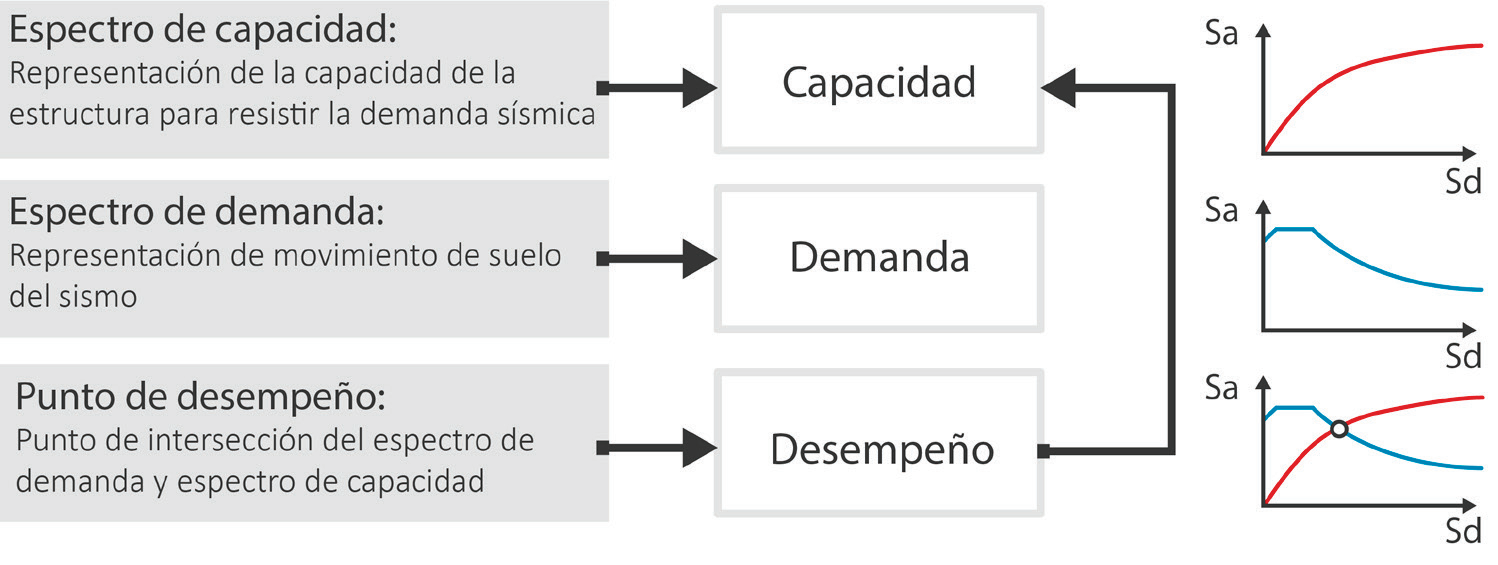
\includegraphics[scale=0.36]{E_IMAGENES/3_Capitulo3/Cap3_Imagen70.png}
	\caption{\centering\footnotesize Cuadro y gráficos que muestran el método N2. Adaptado de \cite{deWaal2009}}
  \figurenote{This is a great figure.}
	\label{Cap3_Figura3}
\end{figure}

\lipsum[19]